	
\renewcommand{\theequation}{\theenumi}
\begin{enumerate}[label=\arabic*.,ref=\thesubsection.\theenumi]
\numberwithin{equation}{enumi}

\item Balance the following chemical equation.
%
\begin{align}
\label{eq:chem_balance}
Fe+H_2O &\rightarrow Fe_3O_4 + H_2
\end{align}
%
\solution Let the balanced version of \eqref{eq:chem_balance} be 
%
\begin{align}
\label{eq:chem_balance_unsol}
x_1Fe+x_2H_2 O &\rightarrow x_3Fe_3 O_4 + x_4H_2
\end{align}
%
which results in the following equations
%
\begin{align}
\begin{split}
\brak{x_1 -3x_3}Fe &= 0
\\
\brak{2x_2 -2x_4}H &= 0
\\
\brak{x_2 -4x_3}O &= 0
\end{split}
\end{align}
which can be expressed as
\begin{align}
\begin{split}
x_1 + 0.x_2 -3x_3 +0.x_4&= 0
\\
0.x_1+2x_2 +0.x_3-2x_4 &= 0
\\
0.x_1+x_2 -4x_3+ 0.x_4 &= 0
\end{split}
\end{align}
%
resulting in the matrix equation
\begin{align}
\label{eq:chem_balance_mat_eq}
\begin{split}
\myvec{
1 & 0 & -3 & 0
\\
0 & 2 & 0 & -2
\\
0 & 1 & -4 & 0
}
\vec{x} &= \vec{0}
\end{split}
\end{align}
%
where
\begin{align}
\vec{x} = \myvec{x_1 \\ x_2 \\ x_3 \\ x_4} 
\end{align}
%\item Solve \eqref{eq:chem_balance_unsol} by row reducing 
%the matrix in \eqref{eq:chem_balance_mat_eq}.
%\\
%\solution  
\eqref{eq:chem_balance_mat_eq} can be row reduced as follows
%
\begin{align}
\label{eq:chem_balance_mat_row}
\myvec{
1 & 0 & -3 & 0
\\
0 & 2 & 0 & -2
\\
0 & 1 & -4 & 0
}
 \xleftrightarrow[]{R_2 \leftarrow \frac{R_2}{2}}
\myvec{
1 & 0 & -3 & 0
\\
0 & 1 & 0 & -1
\\
0 & 1 & -4 & 0
}
\\
 \xleftrightarrow[]{R_3\leftarrow R_3-R_2}
\myvec{
1 & 0 & -3 & 0
\\
0 & 1 & 0 & -1
\\
0 & 0 & -4 & 1
}
\\
 \xleftrightarrow[]{R_1\leftarrow 4R_1-3R_3}
\myvec{
4 & 0 & 0 & -3
\\
0 & 1 & 0 & -1
\\
0 & 0 & -4 & 1
}
\\
 \xleftrightarrow[R_3 \leftarrow -\frac{1}{4}R_3]{R_1\leftarrow \frac{1}{4}}
\myvec{
1 & 0 & 0 & -\frac{3}{4}
\\
0 & 1 & 0 & -1
\\
0 & 0 & 1 & -\frac{1}{4}
}
\end{align}
%
Thus, 
\begin{align}
\label{eq:chem_balance_mat_sol}
x_1 &= \frac{3}{4}x_4, x_2 = x_4, x_3 = \frac{1}{4}x_4
\\
\\
\implies 
\vec{x} &= x_4\myvec{\frac{3}{4} \\ 1 \\ \frac{1}{4} \\ 1}= \myvec{3 \\ 4 \\ 1 \\ 4}
\end{align}
%
upon substituting $x_4 = 4$.
%
\eqref{eq:chem_balance_unsol} then becomes
%
\begin{align}
\label{eq:chem_balance_final}
3Fe+4H_2 O &\rightarrow Fe_3 O_4 + 4H_2
\end{align}

\item Consider the following information regarding the number of men and women workers in the three factories I,II and III

\begin{tabular}{ |c|c|c| } 
\hline
 & Men Workers & Women Workers \\
\hline
\multirow{3}{4em}{I \\II \\III} & 30 & 25\\ 
& 25 & 31 \\ 
&27 & 26 \\ 
\hline
\end{tabular}\\
Represent the above information in the form of a 3 $\times$ 2 matrix. What does the entry
in the third row and second column represent?\\


 \item  If a matrix has 8 elements, what are the possible orders it can have?\\
    \item Construct a 3 $\times$ 2 matrix whose elements are given by $a_{ij}=\frac{1}{2}\abs{i-3j}$\\
    \item \myvec{x+3 &z+4 &2y-7\\-6 &a-1 &0\\b-3 &-21 &0}=\myvec{0 &6 &3y-2\\-6 &-3 &2c+2\\2b+4 &-21 &0}\\
    Find the values of a,b,c,x,y and z.\\
\solution 
 As the two matrices are equal their corresponding entries are also equal. Hence
\begin{align}
x+3&=0 \quad \implies x=-3
\\
z+4&=6 \quad \implies z=2
\\
2y-7&=3y-2 \quad \implies y=-5
\\
a-1&=-3 \quad \implies a=-2
\\
2c+2&=0 \quad \implies c=-1
\\
b-3&=2b+4 \quad \implies b=-7
\end{align}

    \item Find the values of a,b,c and d from the following equation:\\
    \myvec{2a+b &a-2b\\5c-d &4c+3d}=\myvec{4 &-3\\11 &24}\\
\solution 

General equation of conics is 
\begin{align}
    \vec{x}^T\vec{V}\vec{x}+ 2\vec{u}^T\vec{x}+f = 0
    \label{eq:solutions/1/16/eq:1}
\end{align}
Comparing with the equation given,
\begin{align}
\vec{V}=\myvec{\frac{1}{9} & 0 \\ 0 & \frac{1}{16}}\\
\vec{u}=\vec{0}\\
f=-1\\
\mydet{\vec{v}}=\mydet{\myvec{\frac{1}{9} & 0 \\ 0 & \frac{1}{16}}}>0
\end{align}
$\because \abs{\vec{V}}>0$, the given equation is of ellipse.\\
a)The tangents are parallel to the x-axis, hence, their direction and normal vectors, $\vec{m_1}$ and $\vec{n_1}$ are respectively,
\begin{align}
\vec{m_1}=\myvec{1\\0}\\
\vec{n_1}=\myvec{0\\1}
\end{align}
For an ellipse, given the normal vector $\vec{n}$, the tangent points of contact to the ellipse are given by
\begin{align}
    \vec{q}=\vec{V}^{-1}(\kappa \vec{n}-\vec{u})
    \label{eq:solutions/1/16/eq:2}
    =\vec{V}^{-1}\kappa \vec{n}
\end{align}
where
\begin{align}
    \kappa=\pm \sqrt{\frac{\vec{u^T}\vec{V}^{-1}\vec{u}-f}{\vec{n^T}\vec{V}^{-1}\vec{n}}}
    \label{eq:solutions/1/16/eq:2.0.9}\\
   =\pm \sqrt{\frac{-f}{\vec{n^T}\vec{V}^{-1}\vec{n}}}\\
    \vec{V}^{-1}=\myvec{9 & 0 \\ 0 & 16}\\
    \kappa_1=\pm \sqrt{\frac{-(-1)}{\myvec{0 & 1}\myvec{9 & 0 \\ 0 & 16} \myvec{0\\1}}}\\
 \implies \kappa_1=\pm \sqrt{\frac{1}{16}}\\
    \implies \kappa_1=\pm \frac{1}{4}      
\end{align}
From \eqref{eq:solutions/1/16/eq:2} , the point of contact $\vec{q_i}$ are,
\begin{align}
    \vec{q_1}=\myvec{9 & 0 \\ 0 & 16}\frac{1}{4}\myvec{0\\1}\\
    =\myvec{9 & 0 \\ 0 & 16}\myvec{0\\\frac{1}{4}}\\
    =\myvec{0\\4}\\
    \vec{q_2}=\myvec{9 & 0 \\ 0 & 16}\left(-\frac{1}{4}\right)\ \myvec{0\\1}\\
    =\myvec{9 & 0 \\ 0 & 16}\myvec{0\\-\frac{1}{4}}\\
    =\myvec{0\\-4}
\end{align}
b) The tangents are parallel to the y-axis, hence, their direction and normal vectors, $\vec{m_2}$ and $\vec{n_2}$ are respectively,
\begin{align}
\vec{m_2}=\myvec{0\\1}\\
\vec{n_2}=\myvec{1\\0}
\end{align}
Using equation \eqref{eq:solutions/1/16/eq:2.0.9}, the values of $\kappa$ for this case are
\begin{align}
     \kappa_2=\pm \sqrt{\frac{-(-1)}{\myvec{1 & 0}\myvec{9 & 0 \\ 0 & 16} \myvec{1\\0}}}\\
 \implies \kappa_2=\pm \sqrt{\frac{1}{9}}\\
    \implies \kappa_2=\pm \frac{1}{3} 
\end{align}
and from \eqref{eq:solutions/1/16/eq:2} , the point of contact $\vec{q_i}$ are,
\begin{align}
\vec{q_3}=\myvec{9 & 0 \\ 0 & 16}\frac{1}{3}\myvec{1\\0}\\
    =\myvec{9 & 0 \\ 0 & 16}\myvec{\frac{1}{3}\\0}\\
    =\myvec{3\\0}\\
\vec{q_4}=\myvec{9 & 0 \\ 0 & 16}\left(-\frac{1}{3}\right)\ \myvec{1\\0}\\
    =\myvec{9 & 0 \\ 0 & 16}\myvec{-\frac{1}{3}\\0}\\
    =\myvec{-3\\0}
\end{align}
 \begin{figure}[h!]
	\centering
	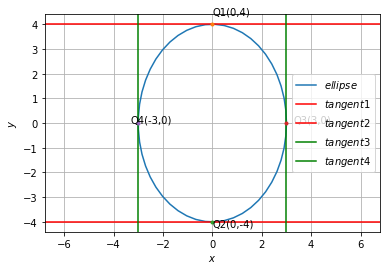
\includegraphics[width=\columnwidth]{./solutions/conics/1/16/ellipse.png}
	\caption{Figure depicting point of contact of tangents of ellipse parallel to x-axis and y-axis}
	\label{eq:solutions/1/16/fig1}
\end{figure}

    \item Given A=\myvec{\sqrt{3} &1 &-1\\2 &3 &0} and B=\myvec{2 &\sqrt{5} &1\\-2 &3 &\frac{1}{2}}, find A+B.\\\solution 

General equation of conics is 
\begin{align}
    \vec{x}^T\vec{V}\vec{x}+ 2\vec{u}^T\vec{x}+f = 0
    \label{eq:solutions/1/16/eq:1}
\end{align}
Comparing with the equation given,
\begin{align}
\vec{V}=\myvec{\frac{1}{9} & 0 \\ 0 & \frac{1}{16}}\\
\vec{u}=\vec{0}\\
f=-1\\
\mydet{\vec{v}}=\mydet{\myvec{\frac{1}{9} & 0 \\ 0 & \frac{1}{16}}}>0
\end{align}
$\because \abs{\vec{V}}>0$, the given equation is of ellipse.\\
a)The tangents are parallel to the x-axis, hence, their direction and normal vectors, $\vec{m_1}$ and $\vec{n_1}$ are respectively,
\begin{align}
\vec{m_1}=\myvec{1\\0}\\
\vec{n_1}=\myvec{0\\1}
\end{align}
For an ellipse, given the normal vector $\vec{n}$, the tangent points of contact to the ellipse are given by
\begin{align}
    \vec{q}=\vec{V}^{-1}(\kappa \vec{n}-\vec{u})
    \label{eq:solutions/1/16/eq:2}
    =\vec{V}^{-1}\kappa \vec{n}
\end{align}
where
\begin{align}
    \kappa=\pm \sqrt{\frac{\vec{u^T}\vec{V}^{-1}\vec{u}-f}{\vec{n^T}\vec{V}^{-1}\vec{n}}}
    \label{eq:solutions/1/16/eq:2.0.9}\\
   =\pm \sqrt{\frac{-f}{\vec{n^T}\vec{V}^{-1}\vec{n}}}\\
    \vec{V}^{-1}=\myvec{9 & 0 \\ 0 & 16}\\
    \kappa_1=\pm \sqrt{\frac{-(-1)}{\myvec{0 & 1}\myvec{9 & 0 \\ 0 & 16} \myvec{0\\1}}}\\
 \implies \kappa_1=\pm \sqrt{\frac{1}{16}}\\
    \implies \kappa_1=\pm \frac{1}{4}      
\end{align}
From \eqref{eq:solutions/1/16/eq:2} , the point of contact $\vec{q_i}$ are,
\begin{align}
    \vec{q_1}=\myvec{9 & 0 \\ 0 & 16}\frac{1}{4}\myvec{0\\1}\\
    =\myvec{9 & 0 \\ 0 & 16}\myvec{0\\\frac{1}{4}}\\
    =\myvec{0\\4}\\
    \vec{q_2}=\myvec{9 & 0 \\ 0 & 16}\left(-\frac{1}{4}\right)\ \myvec{0\\1}\\
    =\myvec{9 & 0 \\ 0 & 16}\myvec{0\\-\frac{1}{4}}\\
    =\myvec{0\\-4}
\end{align}
b) The tangents are parallel to the y-axis, hence, their direction and normal vectors, $\vec{m_2}$ and $\vec{n_2}$ are respectively,
\begin{align}
\vec{m_2}=\myvec{0\\1}\\
\vec{n_2}=\myvec{1\\0}
\end{align}
Using equation \eqref{eq:solutions/1/16/eq:2.0.9}, the values of $\kappa$ for this case are
\begin{align}
     \kappa_2=\pm \sqrt{\frac{-(-1)}{\myvec{1 & 0}\myvec{9 & 0 \\ 0 & 16} \myvec{1\\0}}}\\
 \implies \kappa_2=\pm \sqrt{\frac{1}{9}}\\
    \implies \kappa_2=\pm \frac{1}{3} 
\end{align}
and from \eqref{eq:solutions/1/16/eq:2} , the point of contact $\vec{q_i}$ are,
\begin{align}
\vec{q_3}=\myvec{9 & 0 \\ 0 & 16}\frac{1}{3}\myvec{1\\0}\\
    =\myvec{9 & 0 \\ 0 & 16}\myvec{\frac{1}{3}\\0}\\
    =\myvec{3\\0}\\
\vec{q_4}=\myvec{9 & 0 \\ 0 & 16}\left(-\frac{1}{3}\right)\ \myvec{1\\0}\\
    =\myvec{9 & 0 \\ 0 & 16}\myvec{-\frac{1}{3}\\0}\\
    =\myvec{-3\\0}
\end{align}
 \begin{figure}[h!]
	\centering
	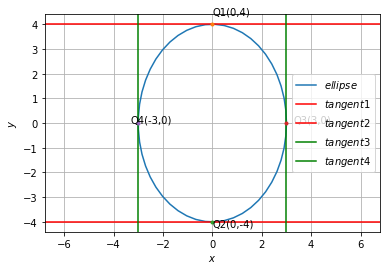
\includegraphics[width=\columnwidth]{./solutions/conics/1/16/ellipse.png}
	\caption{Figure depicting point of contact of tangents of ellipse parallel to x-axis and y-axis}
	\label{eq:solutions/1/16/fig1}
\end{figure}


    \item If A=\myvec{1 &2 &3\\2 &3 &1} and B=\myvec{3 &-1 &3\\-1 &0 &2}, then find 2A-B.\\
    \item If A=\myvec{8 &0\\4 &-2\\3 &6} and B=\myvec{2 &-2\\4 &2\\-5 &1}, then find the matrix X, such that 2A+3X=5B.\\
    \item Find X and Y, if X+Y=\myvec{5 &2\\0 &9} and \\X-Y=\myvec{3 &6\\0 &-1}.\\
    \item Find the values of x and y from the following equation:\\
    2\myvec{x &5\\7 &y-3} + \myvec{3 &-4\\1 &2} = \myvec{7 &6\\15 &14}\\
     
    

    \item Two farmers Ramkishan and Gurcharan Singh cultivates only three
varieties of rice namely Basmati, Permal and Naura. The sale (in Rupees) of these
varieties of rice by both the farmers in the month of September and October are given
by the following matrices A and B. \\
September Sales(in Rupees)\\
   Basmati Permal Naura\\
A =$\myvec{10,000 &20,000 &30,000\\50,000 &30,000 &10,000}$$\myvec{Ramakishan\\Gurucharan Singh}$\\

October sales (in Rupees)\\
  Basmati Permal Naura\\
B=$\myvec{5,000 &10,000 &6,000\\20,000 &10,000 &10,000}$$\myvec{Ramkishan\\Gurucharan Singh}$\\
(i) Find the combined sales in September and October for each farmer in each
variety.\\
(ii) Find the decrease in sales from September to October.\\
(iii) If both farmers receive 2\% profit on gross sales, compute the profit for each
farmer and for each variety sold in October. \\																																															
   
    \item  Find AB, if A=\myvec{6 &9\\2 &3} and B=\myvec{2 &6 &0\\7 &9 &8}.\\
    \item  If A=\myvec{1 &-2 &3\\-4 &2 &5\\} and B=\myvec{2 &3\\4 &5\\2 &1}, then find AB,BA.Show that AB$\neq$BA

   
     \item If A=\myvec{1 &0 \\0 &-1} and  B=\myvec{0 &1\\1 &0}, then find AB,BA. Show that AB$\neq$BA\\
     
   
    \item Find AB, if A=\myvec{0 &-1\\0 &2} and B=\myvec{3 &5\\0 &0}\\
     
   
    \item If A=\myvec{1 &1 &-1\\2 &0 &3\\3 &-1 &2}, B=\myvec{1 &3\\0 &2\\-1 &4} and C=\myvec{1 &2 &3 &-4\\2 &0 &-2 &1}, find\\A(BC),(AB)C and show that (AB)C=A(BC) \\   
    
     \item If A=\myvec{0 &6 &7\\-6 &0 &8\\7 &-8 &0}, B=\myvec{0 &1 &1\\1 &0 &2\\1 &2 &0},C=\myvec{2\\-2\\3}\\Calculate AC,BC and (A+B)C=AC+BC\\

    \item If A=$\myvec{1 &2 &3\\3 &-2 &1\\4 &2 &1}$,then show that $A^3-23A-40I=0$
    
    
    
\item In a legislative assembly election, a political group hired a public relations
firm to promote its candidate in three ways: telephone, house calls, and letters. The
cost per contact (in paise) is given in matrix A as\\ 
Cost per contact\\
A=$\myvec{40 \\100 \\50}\myvec{Telephone \\Housecall \\Letter}$\\
The number of contacts of each type made in two cities X and Y is given by\\
 Telephone  Housecall  Letter\\
B=$\myvec{1000 &500 &5000\\3000 &1000 &10000} \myvec{X \\Y}$. Find the total amount spent by the group in the two cities X and Y. 
\item If A=$\myvec{3 &\sqrt{3} &2\\4 &2 &0}$ and B=$\myvec{2 &-1 &2\\1 &2 &4}$, verify that\\
(i) $(A^{'})^{'}=A$\\ (ii)$(A+B)^{'}=A^{'}+B^{'}$,\\ (iii) $(kB)^{'}=kB^{'}$,where k is any constant.\\
\item If A=$\myvec{-2\\4 \\5}$,B=$\myvec{1 &3 &-6}$, verify that $(AB)^{'}=B^{'}A^{'}$\\
\item Express the matrix B=$\myvec{2 &-2 &-4\\-1 &3 &4\\1 &-2 &-3}$ as the sum of a symmetric and a skew symmetric matrix.\\
\item By using elementary operations,find the inverse of the matrix\\
A=$\myvec{1 &2\\2 &-1}$.\\
\item Obtain the inverse of the following matrix using elementary operations\\
A=$\myvec{0 &1 &2\\1 &2 &3\\3 &1 &1}$.\\
\item Find P$^{-1}$, if it exists, given \\
P=$\myvec{10 &-2\\-5 &1}$.\\
\item If A=$\myvec{\cos\theta &\sin\theta\\ \-sin\theta &\cos\theta}$,\\then prove that $A^{n}=\myvec{\cos\theta &\sin n\theta\\\-sin n\theta &\cos n\theta}$, n $\in$ N.\\
\item If A and B are symmetric matrices of the same order, then show that AB is symmetric if and only if A and B commute,that AB = BA.\\
\item Let A=$\myvec{2 &-1\\3 &4}$, B=$\myvec{5 &2\\7 &4}$, C=$\myvec{2 &5\\3 &8}$. Find a matrix D such that CD-AB=0. 

\end{enumerate}
%\end{document}
    
